\Section{MPEG Encoder in StreamIt}

An MPEG encoder accepts a stream of pictures, or frames, as input.
Each frame is divided into slices and each slice is made up of
macroblocks.  The following process encodes a macroblock.  First, the
encoder performs motion estimation (ME) to determine whether a
macroblock should be predictively coded.  If so, then the encoder uses
motion compensation to reduce the energy in the macroblock.  Next, a
forward DCT (DCT) converts each of the blocks within the macroblock to
the frequency domain.  Then, each of these blocks is quantized (Q).
After quantization, each macroblock is Huffman and run-length encoded
(VLC) and written to a bitstream.  Additionally, the encoder must
perform the decode operation discussed in Section~\ref{sec:dec} so
that motion estimation can be performed using the reconstructed frames
which will be available to the decoder.  Figure~\ref{fig:ec_block}
shows the block diagram of the encode sequence.

\begin{figure}[htbp]
\centerline{ 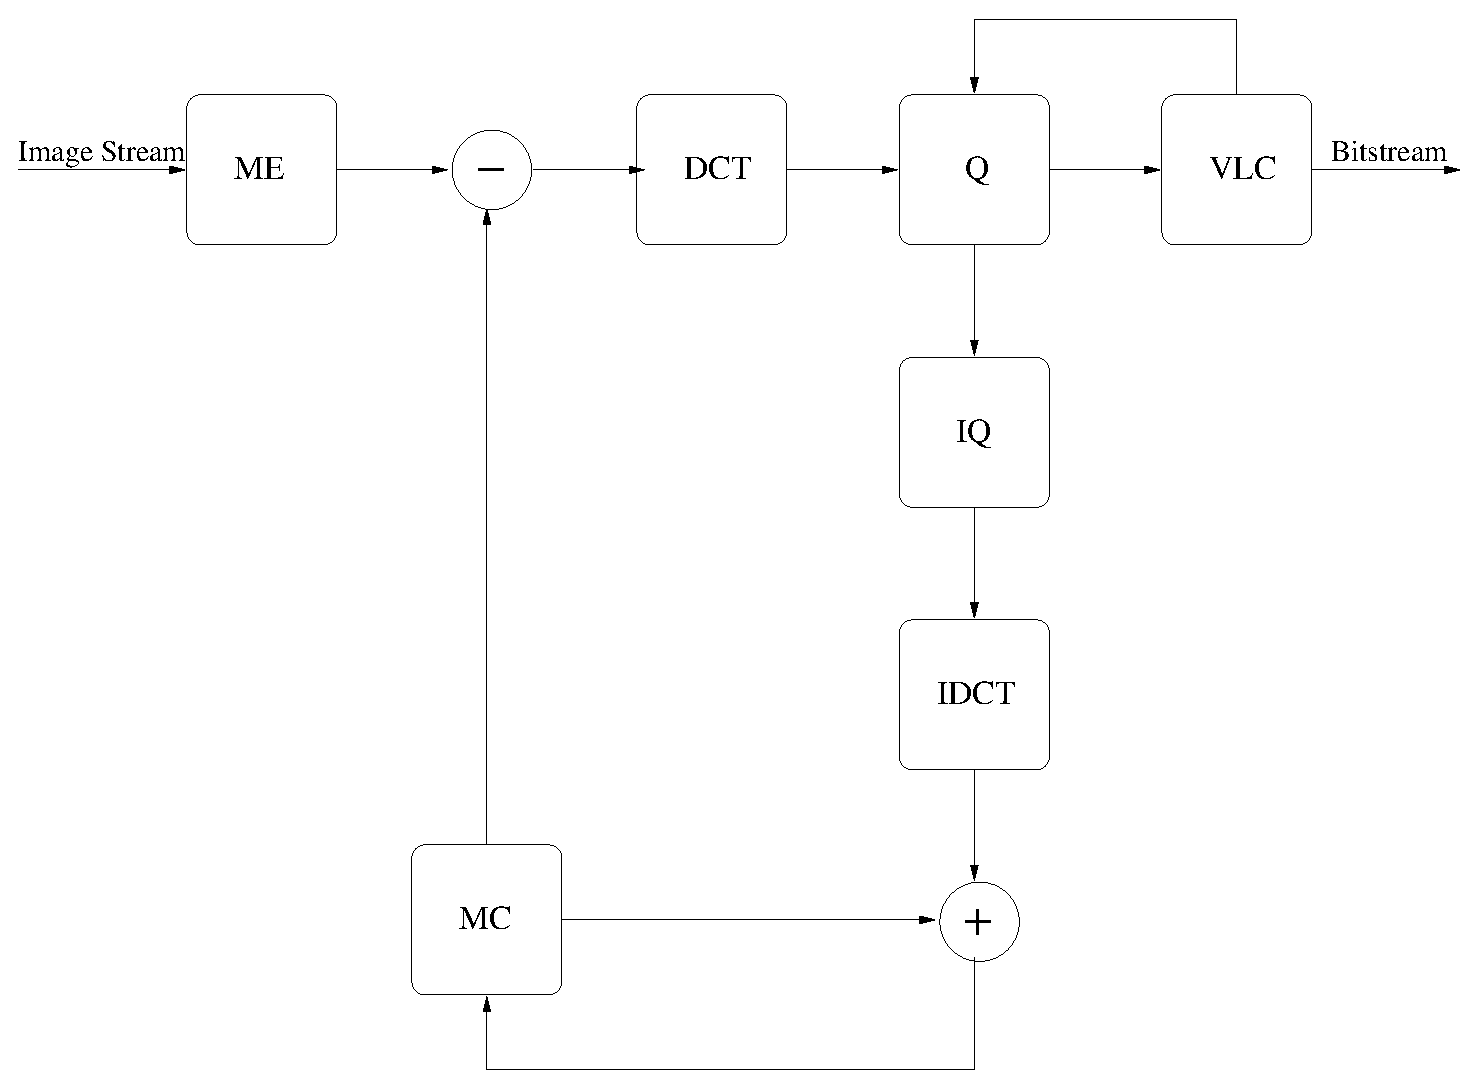
\epsfig{file=ec_block.eps,width=5in}}
\caption{Block diagram of MPEG-2 encode.}
\label{fig:ec_block}
\end{figure}

Our strategy for parallelizing MPEG-2 encoding is based on exploiting
data parallelism among slices.  Slices can be distributed across
streams, and each stream performs all operations independently, except
for motion estimation.

During motion estimation streams need to search through reference
frames to find the best match for the macroblock currently being
encoded.  At this point, inter-stream communication occurs as streams
send each other their locally stored slices of the reference frame.
This communication occurs every time a macroblock is predictively
coded.

The MPEG-2 standard does not specify a minimum or maximum search
window for motion estimation.  It could be as large as the entire
reference frame or as small as a few pixels.  In the case where the
encoder searches the entire reference frame, every stream has to
broadcast its reference slices to all other streams.  This all-to-all
communication can be very inefficient and generally does not scale
well for large numbers of streams.

We exploit the fact that the MPEG-2 standard does not specify a
maximum search window to implement a more efficient communication
scheme. Specifically, we impose a maximum length on motion vectors
produced by our encoder.  This upper bound on motion vector length
limits the potential number of reference macroblocks for a
predictively coded macroblock.  Such an implementation does not
broadcast reference data to all streams, but confines communication to
the sets of streams whose search windows overlap.  Furthermore, by
ensuring that adjacent ranges of macroblocks are allocated to adjacent
streams, this implementation can ensure that communication is local,
as illustrated in Figure~\ref{fig:mb_alloc}.  Such local communication
patterns allow this implementation to scale much more efficiently as
the number of streams grows.

The maximum search window size is a parameter which can be tuned on a
case by case basis.  Larger search windows have the potential for
finding better matches and thus a more compact encoding.  Smaller
search windows limit the amount of communication, offering faster
performance at the cost of either less compression or lower quality
images.  The ideal window size depends on the number of streams, the
size of the frames, and the relative importance of encoder speed and
output quality.

\begin{figure}[htbp]
\centerline{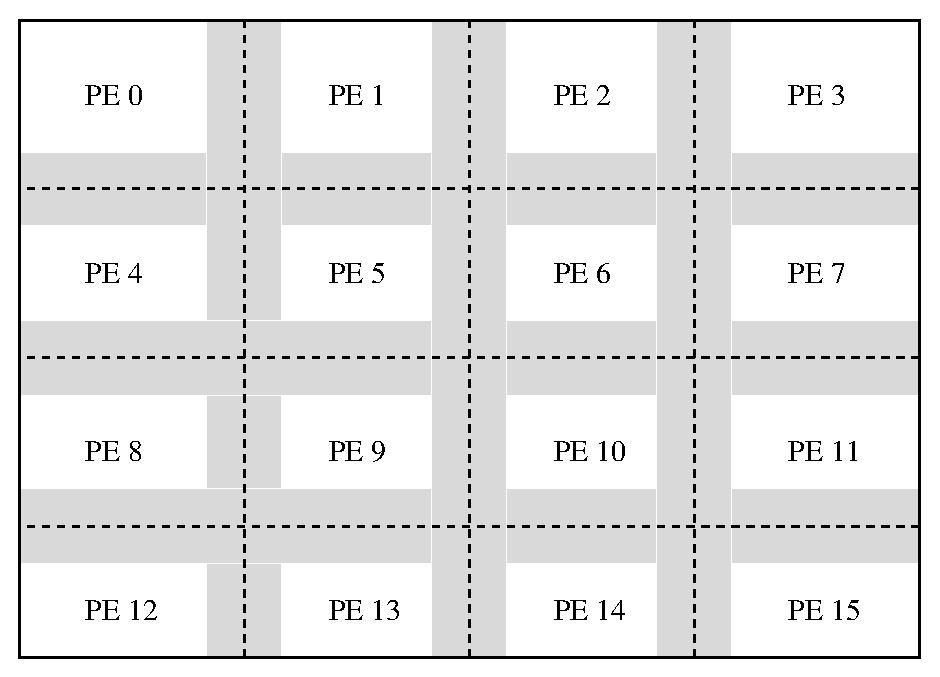
\epsfig{file=mb_alloc.eps,width=5in}}
\caption{Potential allocation of a reference frame among sixteen
streams.  Regions in gray represent reference macroblocks that are
communicated among neighboring streams.  The width of the gray
region represents the maximum motion vector size.}
\label{fig:mb_alloc}
\end{figure}

While using a fixed maximum search window can benefit performance by
reducing the amount of communication overhead, it can be quite
complicated to implement the local communication patterns on actual
hardware.  However, StreamIt provides mechanisms which allow
programmers to expose these local communication patterns to the
compiler.  The compiler handles the burden of allocating streams to
hardware resources and scheduling local communication. The remainder
of this section illustrates these concepts in the context of MPEG-2
encoding.
